\documentclass[11pt,a4paper]{article}

\usepackage{cmap}
\usepackage[margin=2.5cm]{geometry}
\usepackage[T1]{fontenc}
\usepackage[utf8]{inputenc}
\usepackage[brazilian]{babel}
\usepackage{csquotes}
\usepackage[
    backend=biber,
    style=abnt
]{biblatex}

\addbibresource{ref.bib}
\renewcommand*{\bibfont}{\footnotesize}
\usepackage{lmodern}
\usepackage{microtype}
\usepackage{amsmath,amssymb}
\usepackage{enumitem}
\usepackage{array}
\usepackage{booktabs}
\setlength{\aboverulesep}{0.2ex}
\setlength{\belowrulesep}{0.2ex}
\usepackage{xurl}
\usepackage[hidelinks]{hyperref}
\usepackage{graphicx}
\usepackage{placeins}

\setlength{\parindent}{1.25cm}
\setlength{\parskip}{0.35\baselineskip}
\setlength{\emergencystretch}{3em}
\setlist[itemize]{leftmargin=1.2cm,itemsep=0.25em,topsep=0.25em}

\title{\textbf{Comparação de modelos supervisionados em dois cenários de transações Pix: anomalias cadastrais e fraudes comportamentais}}
\author{Éric Silva dos Santos\\Davi Meneses Silva\\Fabio Fonseca Barbosa Gomes\\Celso Barreto da Silva}
\date{}

\begin{document}

\maketitle

\begin{center}
Centro Universitário Jorge Amado (UNIJORGE), Salvador, Bahia, Brasil.\\
\href{mailto:2230200301@unijorge.com.br}{2230200301@unijorge.com.br},
\href{mailto:davi.meneses05@gmail.com}{davi.meneses05@gmail.com}
\end{center}

\begin{abstract}
Este artigo compara Regressão Logística, Random Forest e XGBoost em dois conjuntos sintéticos de transações Pix que representam tarefas distintas. A base de 10 mil registros contém 100 anomalias de cadastro e integridade; a base de 2 milhões, derivada do simulador PaySim e ampliada com registros sintéticos, contém rótulos de fraude comportamental. No teste de 10 mil registros, XGBoost com SMOTE e Random Forest na configuração baseline identificaram 19 das 20 anomalias (F1 de 95,00\% cada); a Regressão Logística com subamostragem identificou oito (F1 de 57,14\%). No teste de 2 milhões, métricas recalculadas das matrizes de confusão indicam F1 de 80,33\% para XGBoost, 72,82\% para Random Forest e 65,16\% para Regressão Logística. Esses resultados devem ser interpretados como exploratórios: no experimento maior, a seleção do modelo usou Average Precision (AP) calculada no teste, o limiar foi ajustado com registros já vistos pelo estimador e as métricas de Random Forest e Regressão Logística ainda precisam ser reconciliadas com as previsões originais. Um ensaio de transferência entre as bases teve recall zero, mas não constitui teste válido de generalização, pois os atributos e o significado dos rótulos não coincidem. Os resultados não demonstram desempenho em transações reais nem redução efetiva de perdas.

\medskip
\noindent\textbf{Palavras-chave:} Detecção de fraudes; anomalias; aprendizado de máquina; Pix; dados sintéticos.
\end{abstract}

\renewcommand{\abstractname}{Abstract}
\begin{abstract}
This paper compares Logistic Regression, Random Forest, and XGBoost across two synthetic Pix transaction datasets representing different tasks. The 10,000-record dataset contains 100 synthetic cadastro and data-integrity anomalies; the 2-million-record dataset, derived from the PaySim simulator and expanded with synthetic records, contains behavioral-fraud labels. On the 10,000-record test set, XGBoost with SMOTE and baseline Random Forest each detected 19 of 20 anomalies (95.00\% F1); Logistic Regression with undersampling detected eight (57.14\% F1). On the 2-million-record test set, metrics recalculated from confusion matrices yielded F1-scores of 80.33\% for XGBoost, 72.82\% for Random Forest, and 65.16\% for Logistic Regression. These results are exploratory: model selection in the larger experiment used Average Precision (AP) on the test set, the decision threshold was tuned on records already seen by the estimator, and Random Forest and Logistic Regression metrics still require reconciliation with the original predictions. A cross-dataset transfer attempt yielded zero recall but is not a valid generalization test because features and label meanings differ. The results do not establish performance on real transactions or actual loss prevention.

\medskip
\noindent\textbf{Keywords:} Fraud detection; anomaly detection; machine learning; Pix; synthetic data.
\end{abstract}

\section{Introdução}

O avanço das tecnologias digitais modificou a forma como pessoas e organizações realizam pagamentos e transferências. No Brasil, o Pix permite movimentar recursos entre contas em poucos segundos e em qualquer dia ou horário. Essa praticidade também aumenta a necessidade de monitorar operações em grande escala e em tempo compatível com a velocidade das transações.

Levantamentos recentes apontam a relevância das fraudes e dos golpes financeiros no Brasil~\cite{Gontijo2025}. Em 2024, as perdas diretas decorrentes de fraudes ultrapassaram R\$ 10,1 bilhões, e foram relatados golpes realizados por canais eletrônicos, cartões de débito e Pix~\cite{Poder3602025}. A engenharia social também pode levar uma pessoa a autorizar uma transferência fraudulenta que, observada isoladamente, se assemelha a uma operação legítima~\cite{cleafy2025social}.

O aprendizado supervisionado pode auxiliar na identificação de padrões em dados transacionais, mas sua avaliação depende da qualidade dos atributos e dos rótulos, do desbalanceamento das classes e do protocolo experimental~\cite{TONG2023110984,MOTIE2024122156}. Em particular, a acurácia pode ser elevada mesmo quando o classificador ignora quase todos os casos minoritários~\cite{10.1145/3343440}. Por isso, a avaliação de fraudes deve considerar tanto os casos positivos detectados quanto os falsos alertas.

Este estudo tem como objetivo comparar o desempenho de três algoritmos de aprendizado de máquina supervisionado sendo eles na identificação de anomalias e fraudes em transações financeiras. Esta análise considera diferentes configurações, incluindo modelos sem e com otimização de hiper parâmetros, bem como a aplicação de estratégias de balanceamento de classes e a ausência dessas estratégias. Os experimentos são conduzidos em dois conjuntos de dados distintos, contendo 10 mil e 2 milhões de registros, respectivamente. O desempenho dos classificadores é analisado por meio de métricas de avaliação, buscando identificar o impacto das diferentes configurações sobre a capacidade avaliativa dos modelos. Também sera discutidas as particularidades de cada conjunto de dados e suas implicações para a interpretação e a comparação dos resultados.

\section{Fundamentação teórica}

\subsection{Aprendizado supervisionado e fraude}

O aprendizado de máquina permite que sistemas computacionais identifiquem padrões presentes nos dados e utilizem essas informações para realizar previsões ou classificações. Dentro desse campo, o aprendizado supervisionado utiliza exemplos previamente classificados durante o treinamento do modelo. Dessa maneira, o algoritmo recebe dados de entrada juntamente com a resposta esperada e procura estabelecer relações que permitam classificar novos registros posteriormente \cite{Mohri2018}.

No contexto das transações financeiras, esse processo pode ser utilizado quando existe um conjunto de dados contendo operações previamente identificadas como legítimas ou fraudulentas. A partir desses exemplos, o modelo procura reconhecer as características associadas a cada classe. \cite{Geron2019} apresenta diferentes algoritmos de classificação que podem ser utilizados em problemas supervisionados, ressaltando que a escolha do método depende das características dos dados e do problema que se pretende resolver.

Na detecção de fraudes, essa característica torna possível comparar diferentes algoritmos utilizando o mesmo conjunto de transações. \cite{Oliveira_2025}, ao realizar um estudo comparativo de métodos de aprendizado de máquina voltados para a detecção de fraude em cartões de crédito, reforça a importância de analisar o comportamento de diferentes modelos diante desse tipo de problema. De forma semelhante, \cite{PreciadoMartinez2025} realizam uma análise comparativa de modelos de aprendizado de máquina aplicados à identificação de transações bancárias fraudulentas, evidenciando que diferentes métodos podem apresentar desempenhos distintos dependendo das características do conjunto de dados utilizado [Preciado Martínez et al. 2025].

\subsection{Algoritmos tabulares comparados}

A Regressão Logística (RL) é uma função usada para problemas binários. É um modelo de referência simples, e seus coeficientes indicam como cada atributo se associa à saída: valores positivos elevam a probabilidade da classe positiva, valores negativos a reduzem. Os coeficientes descrevem associação estatística, não causalidade. Além disso, por ser aditivo e sem termos de interação, o modelo descreve apenas relações simples entre atributos e desfecho, o que limita a representação de regras condicionais complexas \cite{Cox1958, Mohri2018}.

O Random Forest (RF) combina várias árvores treinadas com aleatoriedade em amostras e atributos, agregando suas previsões. A construção em conjunto reduz a dependência de uma árvore individual e permite representar relações não lineares sem exigir uma forma funcional linear explícita. O resultado, porém, varia com a profundidade das árvores, a quantidade de atributos considerados em cada divisão, os pesos de classe e o limiar escolhido. Medidas de importância de atributos devem ser interpretadas com cautela, em especial quando há atributos correlacionados ou derivados uns dos outros\cite{Breiman2001}.

O XGBoost é um método de boosting baseado em árvores: cada etapa acrescenta árvores que buscam reduzir a função de perda do conjunto já construído. A combinação pode modelar interações e regras de decisão complexas, mas sua capacidade também exige controle de profundidade, taxa de aprendizagem, regularização e número de estimadores. Um resultado superior em uma base não permite atribuí-lo automaticamente à arquitetura; amostragem, engenharia de atributos, pesos e limiar também influenciam o desempenho~\cite{xgboost}.

\subsection{Desbalanceamento e métricas}

As fraudes costumam constituir uma parcela pequena das observações. Reamostragem e ponderação de classes podem alterar a aprendizagem do classificador, mas não mudam a prevalência do conjunto de teste, seus efeitos precisam ser avaliados sobre dados que mantenham a distribuição original~\cite{ribeiro2023estrategias,Mqadi_SMOTE}.

Sejam $VP$ os verdadeiros positivos, $VN$ os verdadeiros negativos, $FP$ os falsos positivos e $FN$ os falsos negativos. As métricas usadas neste estudo são:



\begin{align}
    \text{Acurácia} &= \frac{VP+VN}{VP+VN+FP+FN}, \\
    \text{Precisão} &= \frac{VP}{VP+FP}, \\
    \text{Recall} &= \frac{VP}{VP+FN}, \\
    \text{F1-score} &= 2\cdot\frac{\text{Precisão}\cdot\text{Recall}}
    {\text{Precisão}+\text{Recall}}.
\end{align}

Precisão e recall descrevem compromissos diferentes entre alertas corretos e cobertura dos positivos. A curva Precision\textendash{}Recall é particularmente informativa em conjuntos desbalanceados. Neste trabalho, Average Precision (AP) designa a métrica calculada por \texttt{average\_precision\_score}; ela não deve ser confundida com uma área trapezoidal genérica sob a curva Precision\textendash{}Recall~\cite{DavisGoadrich2006}.

A acurácia corresponde à proporção total de classificações corretas. Quando quase todos os registros são negativos, ela pode permanecer alta mesmo se poucos ou nenhum positivo forem encontrados. A precisão responde à pergunta “entre os alertas emitidos, quantos eram positivos?”; o recall responde a “entre os positivos existentes, quantos foram encontrados?”. Uma instituição pode se preocupar com ambas as taxas, mas o ponto de equilíbrio depende da capacidade de investigação, do custo dos erros e do tempo disponível para agir \cite{Geron2019}.

O F1-score é a média harmônica entre precisão e recall. Ele resume o compromisso entre as duas medidas, mas não expressa diretamente o custo monetário de um falso positivo ou de um falso negativo e não incorpora a grande quantidade de verdadeiros negativos. Por isso, dois modelos com F1 semelhante podem gerar cargas de revisão e quantidades de fraudes não detectadas diferentes. A matriz de confusão e as contagens absolutas são necessárias para tornar explícito esse comportamento \cite{Geron2019}.

\subsection{Limiar de decisão e avaliação de escores}

Os classificadores produzem probabilidades estimadas, sendo que a conversão desses valores em uma decisão binária requer um limiar. Reduzir o limiar tende a elevar o recall e também pode aumentar os falsos positivos. Elevá-lo tende a reduzir o volume de alertas, mas pode deixar mais positivos sem detecção. Assim, a comparação de modelos em um único ponto de operação não descreve todo o conjunto de compromissos possíveis.

O limiar que maximiza F1 não é necessariamente o mais adequado para uma instituição. Na ausência de custos definidos para cada tipo de erro, F1 oferece um critério estatístico, não uma função de custo de negócio. Além disso, escolher um limiar não é o mesmo que calibrar probabilidades, sobretudo após ponderação de classes ou reamostragem. Para interpretar probabilidades como riscos, seria necessária uma avaliação específica de calibração em dados com prevalência representativa.

Average Precision resume a ordenação dos positivos ao longo da curva Precision\textendash{}Recall, enquanto precisão, recall e F1 apresentados nas matrizes dependem de um limiar particular. Uma curva pode ajudar a comparar a ordenação dos modelos, mas não substitui a escolha de um ponto operacional nem a avaliação de uma capacidade comum de revisão. Em problemas raros, sua referência aleatória acompanha a baixa prevalência da classe positiva, razão pela qual uma diferença absoluta deve ser lida juntamente com essa taxa-base.

\section{Metodologia}

\subsection{Delineamento e conjuntos de dados}

O estudo tem abordagem quantitativa e compara resultados experimentais já produzidos para três classificadores binários. Foram usados dois conjuntos públicos: o conjunto \textit{PIX banking transaction}, disponibilizado no Kaggle, e o conjunto \textit{PIX Fraud BR}, disponibilizado no Hugging Face~\cite{juniorbuenoPixTransaction,messina2025pixfraudbr}. O segundo é descrito como sintético e derivado do PaySim, simulador de transações financeiras móveis desenvolvido para pesquisa em detecção de fraude~\cite{LopezRojas2016PaySim}.

\begin{table}[htbp]
    \centering
    \caption{Características dos conjuntos e das partições avaliadas.}\label{tab:datasets}%
    \small
    \begin{tabular}{p{3cm}p{5.15cm}p{5.15cm}}
        \toprule
        \textbf{Característica} & \textbf{Cenário de 10 mil} & \textbf{Cenário de 2 milhões} \\
        \midrule
        Registros & 10.000 & 2.000.000 \\
        Positivos totais & 100 anomalias sintéticas (1,00\%) & 15.376 rótulos de fraude (0,7688\%) \\
        Partição de teste & 2.000 registros; 20 positivos & 400.000 registros; 3.075 positivos \\
        Natureza do rótulo & Anomalias cadastrais e de integridade & Padrões financeiros sintéticos rotulados como fraude \\
        Informação característica & Campos cadastrais e transacionais; sem saldos bancários & Valores, saldos antes/depois e atributos derivados \\
        \bottomrule
    \end{tabular}
\end{table}

\FloatBarrier

No conjunto menor, a classe positiva representa anomalias formais sintéticas, não fraudes confirmadas. No conjunto maior, a documentação informa que parte dos registros deriva de PaySim e que o conjunto foi ampliado com geração sintética; os rótulos e algumas distribuições de saldo são condicionados pelas regras do gerador~\cite{messina2025pixfraudbr}. Por isso, o segundo cenário também não equivale a um histórico observado de fraudes Pix reais.

O dataset de 10 mil registros, contém inconsistências de cadastro e integridade, entre elas datas impossíveis, valores zerados, identificadores incompatíveis e divergências de titularidade. A classe positiva, portanto, reúne irregularidades formais inseridas na base, sendo que a presença de uma dessas irregularidades não demonstra necessariamente intenção criminosa, perda financeira ou tentativa de desviar recursos. Os campos disponíveis são predominantemente cadastrais e transacionais, incluindo informações sobre bancos, chaves e horários, mas não os saldos bancários usados na base maior.

No conjunto de 2 milhões, os rótulos positivos se associam a padrões financeiros simulados de esvaziamento de saldo. Os atributos documentados incluem valor e tipo de transferência, momento da operação, saldos do pagador e do recebedor antes e depois da movimentação e razões derivadas de saldo residual. A diferença não é apenas de tamanho: o sinal de classe é produzido por regras distintas e pode estar fortemente associado às variáveis financeiras empregadas pelo simulador. 

Essa distinção orienta a unidade de análise do trabalho. No conjunto menor, o modelo procura reconhecer anomalias explícitas em registros; no conjunto maior, procura separar operações que o processo de simulação rotulou como fraudulentas a partir de estados e movimentações de conta. Os resultados são interpretados dentro de cada tarefa. Diferenças entre seus valores de F1 não medem diretamente qual base “é mais difícil” em sentido universal, pois variam simultaneamente as regras de rotulagem, as escalas monetárias, os atributos e os procedimentos de balanceamento.

\subsection{Particionamento e preparação}

As duas bases foram particionadas em 80\% para treinamento e 20\% para teste: 8.000/2.000 registros na base de 10 mil e 1.600.000/400.000 na de 2 milhões. Como visto em \cite{Geron2019}, foi usado o método \texttt{train\_test\_split} da biblioteca Scikit-Learn já que ela permite uma divisão aleatória e estratificada. Portanto, ela preserva aproximadamente a prevalência das classes.

Na base de 10 mil, os 100 registros positivos correspondem a cerca de 80 exemplos para treinamento e 20 no teste; a base de teste contém ainda 1.980 registros da classe negativa. Na base de 2 milhões, 15.376 rótulos positivos se distribuem entre 12.301 registros de treinamento e 3.075 no teste, enquanto 396.925 registros negativos compõem o teste. Essas contagens são importantes porque as métricas de classificação minoritária variam em função do número absoluto de casos, mesmo quando a prevalência percentual é próxima entre conjuntos.

\begin{figure}[htbp]
    \centering
    \includegraphics[width=\linewidth]{\detokenize{Imagens/comparacao_distribuicao_datasets.png}}
    \caption{Diferença na quantidade de fraudes em cada conjunto}\label{fig:comparacão}%
\end{figure}

Contudo, antes de separar os dados de treinamento e de teste, é necessário fazer um tratamento dos dados como por exemplo na padronização da data de transição que originalmente vem no formato de string, porém que para o modelo conseguir entender os padrões das fraudes, é necessario extrair dados mais detalhados como a hora, dia da semana, se é final de semana ou não

Para o experimento de 2 milhões, uma amostra de 80 mil registros foi usada na exploração de 18 configurações, dividida em subtreino de 60 mil e subvalidação de 20 mil; depois, os modelos foram ajustados na partição de treinamento maior. O pré-processamento inclui imputação e codificação one-hot de variáveis categóricas, com padronização numérica. Tanto para a base de 2 milhões como para a de 10 mil registros, foi treinados e usado os algoritimos usando o dataset base, SMOTE (uma técnica de sobremostragem sintética) e também RandomUnderSampler (técnica de subamostragem aleatória).

Na configuração baseline da base maior, o XGBoost utiliza ponderação da classe positiva e o Random Forest utiliza ponderação balanceada, conforme os artefatos consultados. A subamostragem aleatória reduz exemplos da classe majoritária no treino, o que pode facilitar o ajuste da fronteira com menor custo computacional, mas também descarta observações legítimas potencialmente informativas. A ponderação de classes preserva os registros e altera sua contribuição para a função de perda. O SMOTE produz exemplos minoritários sintéticos por interpolação entre vizinhos, mas a qualidade desses pontos depende da representação e da geometria dos atributos~\cite{Mqadi_SMOTE,ribeiro2023estrategias}.

Em uma avaliação rigorosa, imputação, codificação, escala e reamostragem devem ser ajustadas somente no subconjunto de treinamento de cada validação. O uso de um pipeline reduz o risco de aplicar transformações inconsistentes entre treino e teste. Contudo, o material técnico também registra atributos históricos calculados antes da divisão da base maior; como os registros não foram explicitamente ordenados em sequência temporal antes de calcular essas agregações, a palavra “anterior” não assegura que a informação anteceda cronologicamente a transação. Esse ponto é tratado como risco de dependência e disponibilidade temporal, não como prova automática de vazamento do rótulo.

O SMOTE foi aplicado após a codificação one-hot no pipeline de 2 milhões. Essa ordem pode produzir valores fracionários em atributos categóricos codificados e combinações sintéticas de interpretação discutível; o resultado deve ser entendido como desempenho do pipeline executado, não como validação da plausibilidade dos exemplos gerados.

\subsection{Métricas e protocolo de seleção}

As matrizes de confusão, acurácia, precisão, recall e F1-score foram usadas para descrever o desempenho no ponto de operação indicado nos artefatos. Para a base maior, também foram examinadas as curvas ROC e Precision\textendash{}Recall e os valores de AP registrados na figura. Os limiares exibidos nas matrizes foram 0,283, 0,368 e 0,727 para XGBoost, Random Forest e Regressão Logística no teste de 10 mil; no teste de 2 milhões foram 0,6264, 0,9697 e 0,9697, respectivamente.

As configurações não devem ser lidas como uma comparação controlada apenas da arquitetura. Cada modelo aparece associado a uma estratégia de balanceamento escolhida no experimento, e os limiares também são diferentes. Assim, os resultados descrevem os pipelines selecionados, não o efeito isolado de trocar Regressão Logística por Random Forest ou XGBoost mantendo todos os demais elementos constantes.

Para a base de 10 mil, a seleção por família foi realizada entre as variantes documentadas para esse experimento, e a tabela reporta o pipeline selecionado em cada família, não o melhor valor escolhido retrospectivamente entre quaisquer execuções. Para a base de 2 milhões, a exploração de 18 configurações utilizou a amostra de 80 mil registros; os limiares selecionados foram depois aplicados às previsões mostradas para a partição maior. Os gráficos e matrizes disponíveis são os artefatos de comparação examinados neste trabalho; eles não substituem o armazenamento das previsões individuais necessárias para reproduzir cada métrica.

O protocolo maior apresenta duas limitações relevantes. Primeiro, embora o limiar tenha sido escolhido para maximizar F1, os registros usados para esse ajuste pertenciam ao treinamento final e já haviam sido vistos pelo estimador. Segundo, a escolha do modelo salvo considerou AP no próprio conjunto de teste. Assim, essa partição não permaneceu completamente independente para a seleção final e as métricas devem ser tratadas como exploratórias, possivelmente otimistas, e não como estimativas imparciais de desempenho futuro.

\section{Resultados e discussão}

\subsection{Desbalanceamento das classes}

As duas bases são desbalanceadas, mas a semântica e a prevalência não são iguais: no cenário de 10 mil, 100 de 10.000 registros são anomalias; no de 2 milhões, 15.376 de 2.000.000 são rotulados como fraude. A Figura~\ref{fig:desbalanceamento} mostra a distribuição do primeiro conjunto. No teste dessa base, cada positivo corresponde a cinco pontos percentuais de recall, enquanto no teste de 2 milhões cada um dos 3.075 positivos corresponde a aproximadamente 0,0325 ponto percentual.

\begin{figure}[htbp]
    \centering
    \includegraphics[width=0.78\linewidth]{\detokenize{Imagens/dados desbalanceados.png}}
    \caption{Distribuição das classes no conjunto de 10 mil transações. A classe positiva reúne anomalias sintéticas de cadastro e integridade.}\label{fig:desbalanceamento}%
\end{figure}

\subsection{Resultados no cenário de 10 mil registros}

A Figura~\ref{fig:matriz-10k} e a Tabela~\ref{tab:resultados-10k} mostram os resultados dos pipelines selecionados para a base menor. XGBoost e Random Forest identificaram 19 das 20 anomalias e produziram um falso positivo cada, com F1 de 95,00\%. A Regressão Logística não produziu falsos positivos, mas detectou somente oito anomalias; por isso, sua precisão de 100\% veio acompanhada de recall de 40\% e F1 de 57,14\%. Nesse teste, uma única classificação positiva altera o recall em cinco pontos percentuais, o que limita a resolução das diferenças observadas.

\begin{table}[htbp]
    \centering
    \caption{Métricas e contagens no teste de 2.000 registros.}\label{tab:resultados-10k}%
    \small
    \resizebox{\linewidth}{!}{%
        \begin{tabular}{lrrrrrrrr}
            \toprule
            \textbf{Modelo / estratégia} & \textbf{Acurácia} & \textbf{VN} & \textbf{FP} & \textbf{FN} & \textbf{VP} & \textbf{Precisão} & \textbf{Recall} & \textbf{F1} \\
            \midrule
            XGBoost / SMOTE & 99,90\% & 1.979 & 1 & 1 & 19 & 95,00\% & 95,00\% & 95,00\% \\
            Random Forest / baseline & 99,90\% & 1.979 & 1 & 1 & 19 & 95,00\% & 95,00\% & 95,00\% \\
            Regressão Logística / subamostragem & 99,40\% & 1.980 & 0 & 12 & 8 & 100,00\% & 40,00\% & 57,14\% \\
            \bottomrule
        \end{tabular}%
    }
\end{table}

\begin{figure}[htbp]
    \centering
    \includegraphics[width=\linewidth]{\detokenize{Imagens/01_comparacao_por_modelo-10k (2).png}}
    \caption{Matrizes de confusão dos três pipelines selecionados no teste da base de 10 mil.}\label{fig:matriz-10k}%
\end{figure}

As acurácias de 99,90\% para XGBoost e Random Forest e de 99,40\% para Regressão Logística ilustram por que essa métrica, sozinha, pouco diferencia o comportamento sobre a classe minoritária. No ponto mostrado, o XGBoost e o Random Forest erraram duas transações cada: um falso positivo e um falso negativo. A Regressão Logística acertou todos os registros negativos, mas deixou 12 das 20 anomalias sem identificação. A precisão de 100\% desse modelo deve, portanto, ser lida como ausência de falsos alertas entre os oito casos que sinalizou, e não como detecção completa.

O empate entre XGBoost e Random Forest nesse conjunto não significa que seus escores ou suas fronteiras de decisão sejam idênticos. Os limiares indicados nos artefatos são diferentes, e o conjunto de teste contém somente 20 positivos. Uma diferença de cinco pontos percentuais de recall corresponde a um único registro; por isso, pequenas variações no número de acertos não sustentam, por si só, uma conclusão de superioridade estatística. A amostra permite descrever o resultado observado, mas oferece pouca resolução para estimar estabilidade em outras amostras.

\subsection{Resultados no cenário de 2 milhões}

O teste da base maior reúne 3.075 registros positivos e 396.925 negativos. A Tabela~\ref{tab:resultados-2m} apresenta métricas recalculadas a partir das contagens visíveis nas matrizes de confusão da Figura~\ref{fig:matriz-2m}. Para XGBoost, os números também coincidem com os metadados do modelo. Para Random Forest e Regressão Logística, são valores provisórios extraídos do gráfico, pois não foi possível reconciliá-los com as previsões individuais; o README do experimento registra outros valores para esses dois modelos.

\begin{table}[htbp]
    \centering
    \caption{Resultados recalculados das matrizes no teste de 400.000 registros.}\label{tab:resultados-2m}%
    \small
    \resizebox{\linewidth}{!}{%
        \begin{tabular}{lrrrrrrrr}
            \toprule
            \textbf{Modelo / estratégia} & \textbf{VN} & \textbf{FP} & \textbf{FN} & \textbf{VP} & \textbf{Acurácia} & \textbf{Precisão} & \textbf{Recall} & \textbf{F1} \\
            \midrule
            XGBoost / baseline & 396.353 & 572 & 627 & 2.448 & 99,70\% & 81,06\% & 79,61\% & 80,33\% \\
            Random Forest / baseline & 396.442 & 483 & 1.038 & 2.037 & 99,62\% & 80,83\% & 66,24\% & 72,82\% \\
            Regressão Logística / SMOTE & 395.805 & 1.120 & 1.048 & 2.027 & 99,46\% & 64,41\% & 65,92\% & 65,16\% \\
            \bottomrule
        \end{tabular}%
    }
\end{table}

\begin{figure}[htbp]
    \centering
    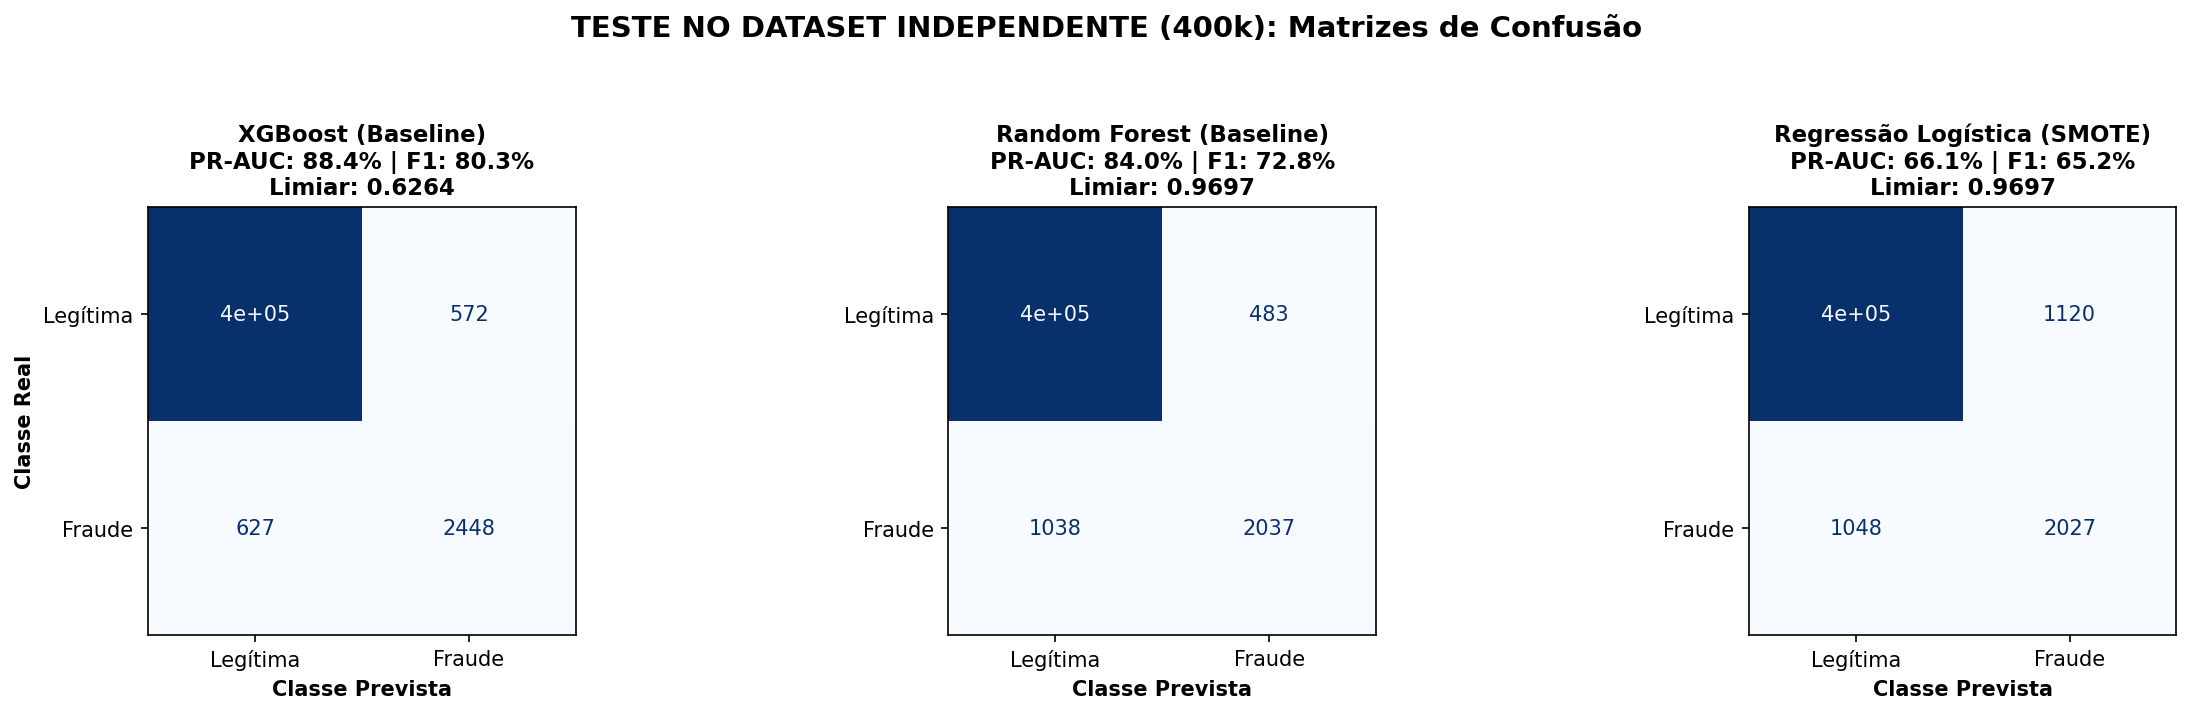
\includegraphics[width=\linewidth]{Imagens/04_matrizes_confusao_teste_2m.png}
    \caption{Matrizes de confusão dos modelos na partição de teste de 400 mil registros. As métricas de Random Forest e Regressão Logística requerem confirmação nas previsões originais.}\label{fig:matriz-2m}%
\end{figure}

Segundo essas contagens, XGBoost apresenta o maior F1 e o maior recall: detecta 2.448 fraudes, mas gera 572 falsos positivos. O Random Forest produz menos falsos positivos (483), porém deixa de identificar 1.038 fraudes. A Regressão Logística detecta quantidade próxima à do Random Forest, mas gera 1.120 falsos positivos. Os limiares são distintos e não foram escolhidos sob uma mesma restrição de capacidade de revisão; portanto, a comparação não estabelece qual modelo é melhor sob um orçamento operacional comum.

Em relação ao total de 3.075 positivos, as contagens correspondem a recalls de 79,61\%, 66,24\% e 65,92\%. Assim, o XGBoost não identifica 627 registros positivos, o Random Forest não identifica 1.038 e a Regressão Logística não identifica 1.048. Para as transações legítimas, as taxas de falsos positivos são aproximadamente 0,144\%, 0,122\% e 0,282\%, respectivamente. Esses percentuais usam como denominador as 396.925 transações negativas; não devem ser confundidos com a proporção de alertas emitidos que são falsos. Esta última é de cerca de 18,94\% para XGBoost, 19,17\% para Random Forest e 35,59\% para Regressão Logística, conforme os totais de alertas das matrizes.

\subsubsection{XGBoost}

No ponto de operação ilustrado, o XGBoost identifica 411 fraudes a mais que o Random Forest e gera 89 falsos positivos adicionais. Em comparação com a Regressão Logística, identifica 421 fraudes a mais e produz 548 falsos positivos a menos. Esses contrastes ajudam a explicitar o compromisso entre detecção e carga de revisão, mas não estabelecem uma ordenação definitiva: os limiares diferem e a seleção do modelo foi condicionada ao AP observado no teste. Os 627 falsos negativos restantes continuam relevantes; o F1 mais alto não elimina a necessidade de investigar que tipos de operação o modelo deixa passar.

\subsubsection{Random Forest}

O Random Forest gera o menor número de falsos positivos entre as matrizes disponíveis e, portanto, também o menor número total de alertas. Isso pode ser atraente quando a capacidade de análise manual é limitada. Em contrapartida, sua cobertura de fraude é inferior à do XGBoost no limiar apresentado: 1.038 positivos não são detectados. Não se pode concluir que essa diferença decorra apenas da arquitetura da floresta, pois profundidade, pesos, amostragem, atributos e corte de decisão também determinam a resposta do classificador.

Uma comparação orientada à operação deveria avaliar os modelos sob a mesma quantidade máxima de alertas, o mesmo orçamento de revisão ou uma taxa de falsos positivos fixada previamente. As matrizes atuais não aplicam essa restrição comum. Logo, o fato de o Random Forest sinalizar menos registros não demonstra, isoladamente, maior eficiência: é necessário considerar quantas fraudes são encontradas dentro do mesmo volume de revisão.

\subsubsection{Regressão Logística}

A Regressão Logística sinaliza 3.147 operações, quantidade superior às 3.020 do XGBoost e às 2.520 do Random Forest, apesar de identificar praticamente o mesmo número de fraudes que o Random Forest. Aproximadamente 35,59\% de seus alertas são falsos positivos. Uma fronteira linear no espaço dos atributos transformados pode ser menos flexível para certas interações entre valores e saldos, mas os dados disponíveis não permitem atribuir causalmente o resultado a essa característica. A estratégia SMOTE, a escala, a regularização e o limiar também participam do comportamento observado.

\subsubsection{Leitura das curvas Precision\textendash{}Recall}

As curvas mostram como precisão e recall variam quando o limiar muda. A curva do XGBoost permanece acima das demais em grande parte da faixa exibida, compatível com os valores indicados no gráfico como “PR-AUC”: aproximadamente 88,41\% para XGBoost, 84,00\% para Random Forest e 66,05\% para Regressão Logística. Neste artigo, esses valores são interpretados como AP, conforme o método de cálculo descrito no material técnico. A prevalência positiva do teste, cerca de 0,77\%, também aparece como referência.

AP mede a ordenação global dos escores, não uma probabilidade calibrada nem a qualidade de um corte único. Somente o valor de XGBoost foi confirmado nos metadados consultados; os valores de Random Forest e Regressão Logística ainda precisam ser verificados nas previsões originais. Além disso, a escolha do vencedor pelo AP calculado no teste transforma a figura em parte do processo de seleção. Ela é útil para descrever os resultados, mas não constitui avaliação imparcial do modelo escolhido.

\begin{figure}[htbp]
    \centering
    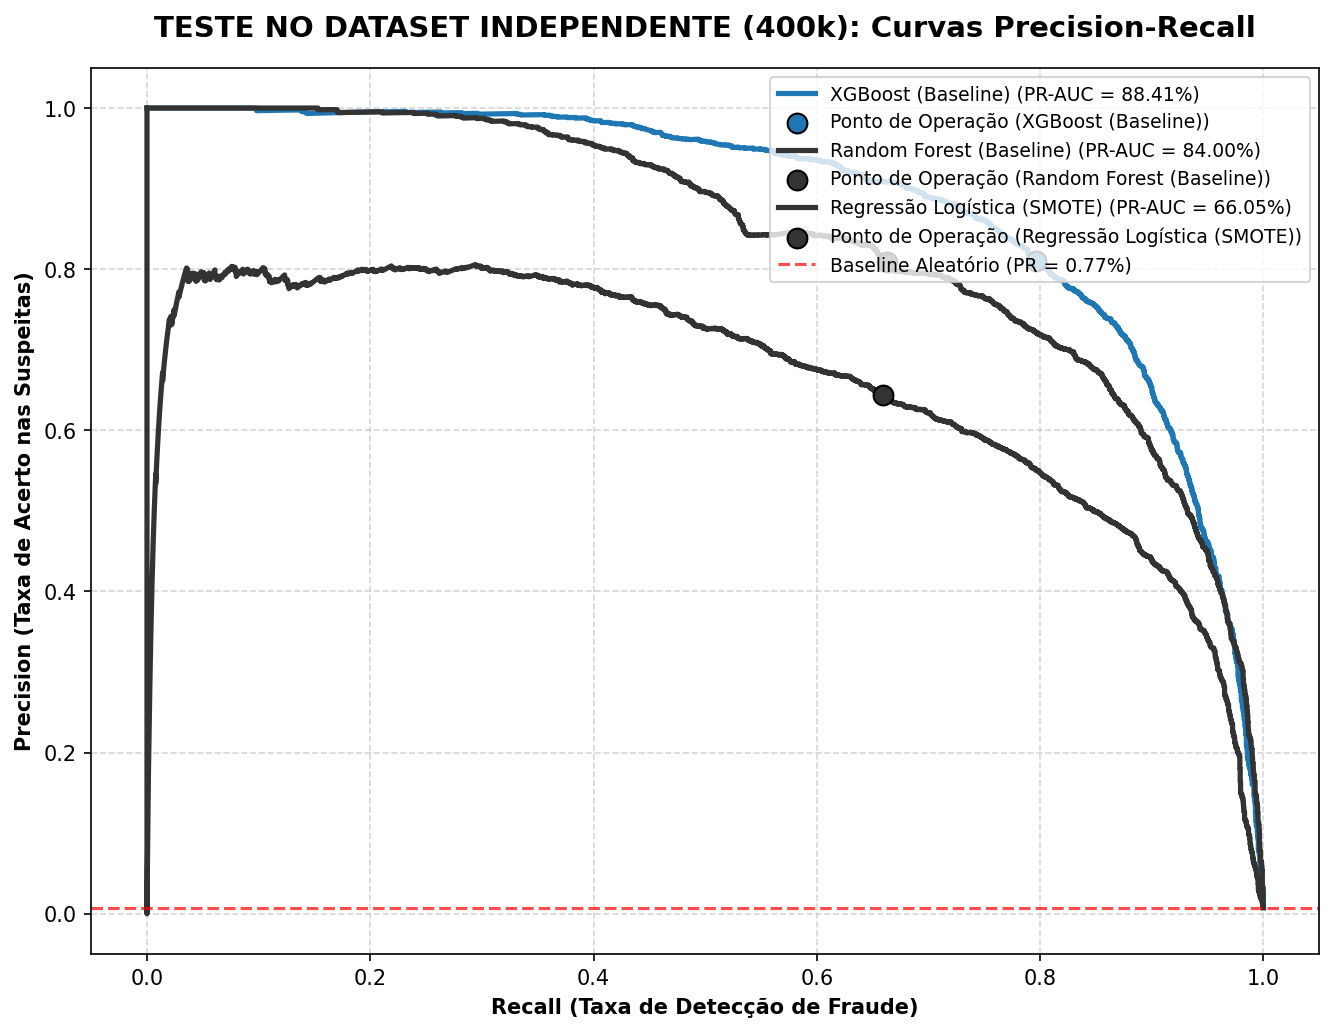
\includegraphics[width=0.82\linewidth]{Imagens/06_curvas_precision_recall_teste_2m.png}
    \caption{Curvas Precision\textendash{}Recall na partição de teste de 400 mil registros. Os valores reportados no gráfico são interpretados como Average Precision (AP), não como área trapezoidal.}\label{fig:curva-pr}%
\end{figure}

Embora as acurácias excedam 99\%, uma regra que classificasse todos os registros como legítimos já obteria aproximadamente 99,23\% nesse teste, com recall nulo. Esse contraste confirma que acurácia isolada é insuficiente para avaliar a detecção de uma classe com prevalência inferior a 1\%.

\subsection{Síntese comparativa entre os cenários}

A Tabela~\ref{tab:sintese-cenarios} reúne o F1 observado em cada base para facilitar a leitura da posição relativa dos modelos. A diferença em pontos percentuais é meramente descritiva: os conjuntos usam atributos, semânticas de rótulo, estratégias de balanceamento e procedimentos de seleção distintos.

\begin{table}[htbp]
    \centering
    \caption{Síntese descritiva do F1 nos dois cenários experimentais.}\label{tab:sintese-cenarios}%
    \small
    \begin{tabular}{lrrr}
        \toprule
        \textbf{Modelo} & \textbf{F1: 10 mil} & \textbf{F1: 2 milhões} & \textbf{Diferença descritiva} \\
        \midrule
        XGBoost & 95,00\% & 80,33\% & $-14,67$ p.p. \\
        Random Forest & 95,00\% & 72,82\% & $-22,18$ p.p. \\
        Regressão Logística & 57,14\% & 65,16\% & $+8,02$ p.p. \\
        \bottomrule
    \end{tabular}
\end{table}

Na base menor, XGBoost e Random Forest empatam no resultado selecionado, enquanto a Regressão Logística apresenta recall mais baixo. Na base maior, o XGBoost tem F1 7,51 pontos percentuais acima do Random Forest e 15,17 pontos acima da Regressão Logística, segundo as matrizes disponíveis. Essas diferenças não isolam o impacto do volume: a classe positiva de 10 mil representa inconsistências cadastrais, e a classe de 2 milhões representa padrões financeiros simulados. Também mudam as proporções e os tipos de atributos, a estratégia de balanceamento e a robustez documental das métricas.

O teste de 10 mil tem resolução muito limitada para comparações: cada positivo move o recall em cinco pontos percentuais. A base de 2 milhões contém mais casos positivos e permite incrementos menores, mas isso não remove a seleção de modelo usando AP no teste, a possível dependência entre registros sintéticos nem os demais riscos de validação. Nenhum teste de significância foi reportado; assim, os números sustentam uma descrição dos artefatos avaliados, não uma afirmação sobre diferenças populacionais entre algoritmos.

\subsection{Ensaio exploratório de transferência entre bases}

O material de apoio relata que aplicar o modelo treinado no conjunto de 2 milhões ao conjunto de 10 mil classificou todos os registros como legítimos: a acurácia aparente foi 99\%, mas o recall das 100 anomalias foi zero. Esse resultado não deve ser apresentado como prova de generalização ou de falha universal de transferência. A base menor não contém atributos de saldo usados pelo modelo maior e seus rótulos representam anomalias formais, enquanto a base de 2 milhões representa padrões financeiros simulados. A operação é, portanto, um diagnóstico de incompatibilidade entre domínios e definições de classe, não uma validação cruzada entre conjuntos equivalentes.

A acurácia de 99\% nesse ensaio decorre da distribuição da base menor: prever toda transação como legítima acerta os 9.900 registros negativos e erra as 100 anomalias. Esse exemplo demonstra, de forma concreta, como uma acurácia aparentemente alta pode coexistir com inutilidade completa para a classe-alvo. O resultado de transferência também é condicionado ao processamento de colunas ausentes, que a documentação descreve como preenchidas pela imputação do pipeline; quando os atributos relevantes de saldo não existem no conjunto de destino, imputá-los não recupera a informação ausente.

Há ainda uma discrepância de escala monetária entre as bases. O material de apoio informa valores de até R\$ 4.999,00 no cenário de 10 mil, enquanto as fraudes simuladas da base maior têm valor médio muito superior, da ordem de R\$ 1,46 milhão. Essa diferença, associada à ausência de saldos no conjunto menor, oferece uma explicação plausível para o colapso da transferência, mas não permite separar o efeito de escala do efeito de semântica do rótulo, composição de atributos e estratégia de imputação. Para estudar transferibilidade, seria necessário construir um problema comum, com variáveis comparáveis, rótulos equivalentes e protocolo de avaliação explicitamente definido.

\subsection{Leitura financeira exploratória}

Para o XGBoost, os metadados registram aproximadamente R\$ 3,96 bilhões em transações rotuladas como fraude e sinalizadas corretamente, R\$ 450 milhões em volume rotulado como fraude não detectado e R\$ 453 milhões em transações legítimas sinalizadas. Esses montantes são valores simulados presentes na base, não perdas reais evitadas, dinheiro recuperado ou custo efetivo dos falsos positivos. Como os valores monetários dos outros modelos não foram reconciliados com suas previsões, eles não são usados para uma comparação financeira entre algoritmos.

O volume corretamente sinalizado representa cerca de 89,78\% do montante atribuído às transações positivas no teste, proporção superior ao recall por quantidade de 79,61\%. No conjunto simulado, portanto, o modelo recupera uma parcela maior do valor rotulado do que do número de registros positivos; essa diferença sugere que os casos de maior valor estão mais frequentemente entre os detectados. A inferência limita-se à distribuição criada pelo gerador e não comprova que um sistema real protegeria a mesma proporção do dinheiro movimentado.

Uma análise econômica operacional exigiria estimar consequências que não estão disponíveis nesses artefatos: probabilidade de o alerta impedir a transação, possibilidade de recuperação após a liquidação, custo de análise humana, atrito imposto a clientes legítimos e custo de oportunidade dos falsos negativos. O volume de operações legítimas sinalizadas não é, por si só, prejuízo financeiro, assim como o valor de uma operação rotulada como fraude não equivale automaticamente à perda líquida que seria evitada. Por esse motivo, não se descrevem os números como “capital protegido” ou “fraude bloqueada”.

\subsection{Limitações e implicações}

Os resultados dependem de bases sintéticas. A documentação do conjunto de 2 milhões descreve a geração de registros adicionais por bootstrap com ruído e a criação de distribuições de saldo condicionadas ao rótulo. Dessa forma, os modelos podem aprender regularidades próprias do mecanismo de geração; isso não assegura que mantenham o desempenho em fraude real. A ampliação sintética também exige verificar similaridade entre exemplos de treino e teste.

\subsubsection{Validade dos rótulos e dos dados}

No conjunto de 10 mil, as anomalias são inserções sintéticas de integridade e cadastro. Um classificador pode aprendê-las por sinais explícitos — como um campo inválido ou um valor extremo — sem aprender a reconhecer fraude financeira ou engenharia social. No conjunto de 2 milhões, os rótulos foram produzidos em um ambiente simulado, e a documentação descreve que saldos e exemplos foram gerados em relação à classe. O modelo pode, assim, reproduzir as regularidades do mecanismo que criou os rótulos. Essa possibilidade não invalida o experimento como exercício metodológico, mas restringe a interpretação: trata-se da separação entre classes definidas por esses dados, não de evidência direta sobre fraude em uma instituição.

A geração por reamostragem e ruído também levanta uma questão de independência entre observações. Se variantes muito próximas do mesmo registro aparecem simultaneamente no treino e no teste, a avaliação aleatória pode refletir reconhecimento de padrões repetidos, e não generalização para eventos novos. O material consultado recomenda investigar essa sobreposição; os resultados apresentados não incluem uma análise de duplicidade ou de vizinhança entre partições. Uma auditoria futura deveria comparar hashes, identificadores pseudonimizados e distâncias entre registros, além de fazer partições agrupadas quando houver entidade de origem comum.

\subsubsection{Validade temporal e disponibilidade dos atributos}

O particionamento aleatório não avalia a generalização temporal nem para clientes inéditos. Além disso, atributos de saldo posterior à transação podem não estar disponíveis no instante em que uma instituição precisaria decidir bloquear uma operação; sua origem e disponibilidade temporal precisam ser auditadas antes de qualquer interpretação operacional. A seleção baseada em AP no teste e o ajuste do limiar em registros vistos pelo estimador podem tornar as métricas otimistas. A subvalidação usada na busca das configurações continha cerca de 154 positivos, e não foram apresentados intervalos de confiança ou repetições independentes.

A ausência de ordenação cronológica garantida torna especialmente importante auditar variáveis históricas. Contagens, médias e medianas por pagador calculadas antes da divisão aleatória podem incorporar relações entre registros que depois aparecem em partições distintas. Mesmo quando uma variável exclui o valor da própria linha, ainda é necessário confirmar que seus demais componentes eram observáveis antes do instante de cada transação. Uma avaliação temporal deve reconstruir esses atributos em ordem de evento e comparar treino em períodos anteriores com teste em um período posterior.

Também é necessário separar desempenho de classificação e viabilidade de intervenção. Saldos posteriores podem ajudar a descrever o que aconteceu depois da movimentação, mas não necessariamente estão disponíveis para uma decisão preventiva em tempo real. Antes de qualquer uso prospectivo, cada coluna precisa ser classificada segundo o momento em que passa a existir, sua fonte e se depende de um evento posterior ao alerta.

\subsubsection{Seleção, limiar e incerteza}

O ajuste de limiar no conjunto maior usa registros que também participaram do ajuste do estimador, o que pode favorecer um corte otimista. Separadamente, a seleção do vencedor pelo maior AP do teste significa que o teste influenciou a decisão sobre qual algoritmo seria apresentado como melhor. Esses mecanismos de reutilização são distintos: um afeta a escolha do limiar; o outro afeta a comparação e escolha do modelo. Ambos recomendam tratar os números como exploratórios e reservar uma nova partição intocada para uma avaliação confirmatória.

As 18 configurações foram examinadas em uma subvalidação de 20 mil registros com cerca de 154 positivos. Embora o teste de 400 mil contenha mais exemplos minoritários, o tamanho da partição final não corrige a seleção prévia feita no próprio teste. Além disso, os boxplots de configurações diferentes não são repetições independentes do experimento e não constituem intervalos de confiança. Para quantificar a variabilidade, seria necessário repetir partições ou realizar reamostragem estatística que respeitasse a unidade independente dos dados, como usuário ou período.

\subsubsection{Consistência e reprodutibilidade}

Há também uma inconsistência documental entre as métricas de Random Forest e Regressão Logística publicadas no README e as que se recalculam das matrizes disponíveis. Até que sejam recuperadas as previsões individuais e reproduzidos os cálculos com um único protocolo, os valores desses modelos devem ser considerados provisórios. O SMOTE após one-hot encoding e a falta de comparação sob uma mesma taxa de falsos positivos são limitações adicionais.

Uma trilha reprodutível deveria armazenar, para cada execução, a versão exata do conjunto de dados, identificadores das partições, semente aleatória, lista de atributos, transformações, estratégia de balanceamento, hiperparâmetros, limiar e escores contínuos de teste. As matrizes e as métricas poderiam então ser recalculadas a partir do mesmo vetor de previsões, evitando que números de execuções distintas sejam misturados em tabelas ou imagens. O material disponível não contém as previsões individuais necessárias para executar essa reconciliação nesta revisão.

O uso de SMOTE após codificação one-hot demanda uma verificação adicional. A interpolação entre vetores categóricos binários pode gerar coordenadas fracionárias que não correspondem a categorias observadas. Em dados mistos, seria necessário avaliar uma estratégia compatível com variáveis categóricas ou comparar a reamostragem com ponderação da função de perda. A ausência dessa verificação não altera as contagens publicadas, mas limita a interpretação do que o modelo aprendeu.

Uma avaliação confirmatória deveria separar dados para ajuste de hiperparâmetros, seleção do limiar e teste final; escolher o modelo sem consultar o teste; validar por tempo e, quando pertinente, por usuário; auditar variáveis disponíveis no momento da decisão; reconciliar as previsões e métricas; e avaliar os modelos sob custos ou capacidade de revisão explicitamente definidos. Também seriam necessários dados reais e validação externa para sustentar conclusões sobre operações Pix em produção.

\subsection{Protocolo sugerido para uma avaliação confirmatória}

Uma próxima etapa pode tratar os problemas identificados como requisitos de desenho experimental, e não apenas como ressalvas posteriores. A Tabela~\ref{tab:protocolo-futuro} resume os principais riscos e os controles recomendados para uma avaliação mais forte.

\begin{table}[htbp]
    \centering
    \caption{Riscos metodológicos e controles recomendados para estudos futuros.}\label{tab:protocolo-futuro}%
    \small
    \begin{tabular}{>{\raggedright\arraybackslash}p{3.6cm}>{\raggedright\arraybackslash}p{4.4cm}>{\raggedright\arraybackslash}p{5.1cm}}
        \toprule
        \textbf{Risco observado} & \textbf{Consequência possível} & \textbf{Controle recomendado} \\
        \midrule
        Seleção de modelo pelo teste & Desempenho final otimista & Separar desenvolvimento e teste final intocado \\
        Ajuste do limiar em treino já visto & Corte superajustado aos exemplos & Usar previsões fora da amostra ou validação exclusiva \\
        Partição aleatória de dados temporais & Não mede desempenho futuro & Treinar em períodos anteriores e testar em período posterior \\
        Registros derivados ou repetidos & Similaridade entre treino e teste & Agrupar por origem e auditar duplicidade/vizinhança \\
        Atributos pós-transação & Informação indisponível no momento de ação & Auditar cada variável por instante de disponibilidade \\
        Métricas operacionais divergentes & Comparação não reproduzível & Recalcular de previsões individuais versionadas \\
        \bottomrule
    \end{tabular}
\end{table}

O protocolo poderia reservar uma partição de desenvolvimento para seleção de atributos e hiperparâmetros, uma validação independente para escolher o limiar e um teste final utilizado uma única vez. Em um estudo prospectivo, a separação temporal deveria ser prioritária; se a decisão visada for sobre clientes sem histórico prévio, seria necessário complementar com uma partição agrupada por entidade. Se existirem os dois objetivos, os resultados deveriam ser reportados separadamente, pois respondem a perguntas distintas.

Antes do treinamento, cada atributo deveria ser classificado como disponível antes da autorização, disponível durante o processamento ou conhecido somente após a liquidação. Variáveis históricas precisam ser reconstruídas em ordem cronológica, sem utilizar observações futuras da mesma conta. A seleção entre algoritmos deve ocorrer exclusivamente no desenvolvimento; o limiar deve ser ajustado em validação separada e o teste final precisa permanecer cego a ambas as decisões.

Por fim, a comparação operacional deveria fixar uma capacidade máxima de revisão ou uma taxa de falso positivo aceitável, e apresentar junto a ela recall, precisão, número de fraudes não detectadas e distribuição dos erros por faixa de valor e perfil. A calibração dos escores, a estabilidade entre períodos e a incerteza das métricas deveriam ser avaliadas em blocos que preservem a dependência entre transações do mesmo cliente. Somente depois dessas etapas seria apropriado discutir implantação piloto, sempre com revisão humana, monitoramento de deriva e critérios de interrupção definidos previamente.

\section{Considerações finais}

O estudo comparou três classificadores em dois cenários sintéticos que não representam a mesma tarefa. No conjunto de 10 mil registros, XGBoost com SMOTE e Random Forest baseline obtiveram F1 de 95,00\%, identificando 19 das 20 anomalias; a Regressão Logística com subamostragem obteve F1 de 57,14\%. No conjunto de 2 milhões, as matrizes disponíveis indicam F1 de 80,33\% para XGBoost, 72,82\% para Random Forest e 65,16\% para Regressão Logística, com ressalvas de consistência para os dois últimos.

No conjunto menor, a Regressão Logística exemplifica que precisão elevada pode coexistir com baixa cobertura: seus oito alertas eram corretos, mas 12 das 20 anomalias não foram identificadas. No cenário maior, o XGBoost apresenta o maior F1 e recall entre as contagens disponíveis, enquanto o Random Forest produz menos falsos positivos e a Regressão Logística tem maior proporção de alertas incorretos. Esses perfis apontam compromissos distintos, e não uma solução única independente de capacidade operacional.

O XGBoost foi o modelo com melhor F1 nas contagens observadas da base maior, mas isso não basta para afirmar superioridade geral: houve seleção usando AP no teste, reutilização de dados de treinamento no ajuste do limiar, inconsistências entre artefatos e limitações de dados sintéticos. Da mesma forma, o resultado de recall zero na transferência para a base de 10 mil reflete tarefas e atributos incompatíveis, não uma estimativa válida de generalização.

Conclui-se que os resultados são evidências exploratórias restritas aos conjuntos e aos procedimentos descritos. Eles não isolam o efeito do tamanho da amostra, não demonstram eficácia em dados financeiros reais e não quantificam perdas evitadas em produção. A comparação entre bases deve ser compreendida como comparação entre tarefas, e não como experimento controlado sobre o benefício de ampliar a quantidade de dados.

Como contribuição metodológica, o trabalho evidencia que a definição do rótulo, a disponibilidade temporal dos atributos, o modo de seleção do limiar e a separação entre treino, validação e teste são tão importantes quanto a escolha do algoritmo. A prioridade para trabalhos futuros é reconciliar as previsões, construir um protocolo de avaliação independente e temporal, comparar os modelos sob uma capacidade comum de revisão e testar seu desempenho em dados representativos do contexto de uso. Apenas resultados obtidos nessas condições poderão sustentar recomendações sobre uma aplicação real de detecção de fraude em transações Pix.

\addcontentsline{toc}{section}{Referências}
\printbibliography%

\end{document}
